
% Este documento LaTeX fue dise�ado por profesores  del Departamento de Matem�ticas
% de la Universidad de Antioqua (http://ciencias.udea.edu.co/). Usted puede modificarlo
% y personalizarlo a su gusto bajo los t�rminos de la licencia de documentaci�n libre GNU.
% http://es.wikipedia.org/w/index.php?title=Licencia_de_documentaci%C3%B3n_libre_de_GNU&oldid=15717448

%\documentclass[serif,9pt]{beamer}
%\setbeamertemplate{navigation symbols}{}

%\setbeamercolor{frametitle}{fg=black,bg=white}
%\setbeamercolor{title}{fg=black,bg=yellow!85!orange}
%\usetheme{AnnArbor}

%\documentclass{beamer}

\documentclass[serif,9pt]{beamer}

\usetheme{Frankfurt}

%\usefonttheme{progressbar}
%\useoutertheme{progressbar}
%\useinnertheme{progressbar}
%\usecolortheme{crane}
\usepackage[latin1]{inputenc}
\usepackage[spanish]{babel}
\usepackage{graphicx}
\usepackage{ragged2e}
\usebackgroundtemplate{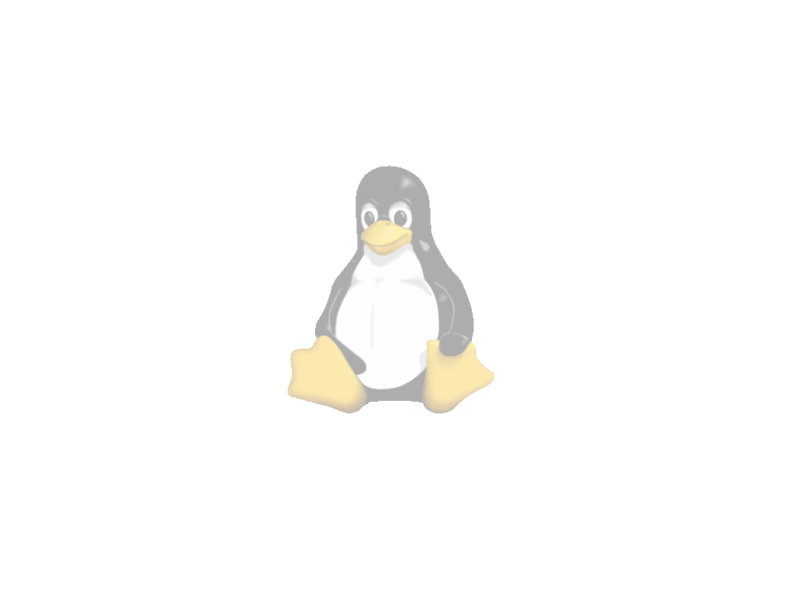
\includegraphics[width= \paperwidth, height=\paperheight]{img/fondo.png}}
%\logo{\includegraphics[scale=0.4]{Tux}}

\beamersetuncovermixins{\opaqueness<1>{25}}{\opaqueness<2->{15}}
\begin{document}

\title[Evidencia Digital]{{\bfseries {\LARGE ``Evitando la Falsificaci�n/ Alteraci�n de evidencia Digital.''}%
  }}
\author[DESEIN 2012]{\LARGE Jose Moruno Cadima }
\institute[]
\bigskip
\bigskip
\\
\\

\date[Noviembre, 2012]{ Twitter:@sniferl4bs \\ www.sniferl4bs.blogspot.com}
\begin{frame}[plain]
\titlepage
\end{frame}

\begin{frame}\frametitle{Que veremos}\tableofcontents
\end{frame}


\section{Introducci�n}


\subsection{Que es la Evidencia}

\begin{frame}\frametitle{Evidencia}


\begin{itemize}
\item Delito.\pause
\item Proceso de investigaci�n.\pause
\item Evidencia. \pause
\end{itemize}

Es una certeza que resulta amigable y  que no se puede dudar.

\begin{itemize}
\item ``Su rostro es la evidencia m�s clara de la violencia de g�nero.''
\end{itemize}

\end{frame}



\subsection{Evidencia Digital}

\begin{frame}\frametitle{Evidencia Digital}

\begin{itemize}
\item Actualmente la evidencia, es presentada en medios digitales...
\end{itemize}
\end{frame}


\begin{frame}\frametitle{Evidencia Digital}
\begin{figure}[h]
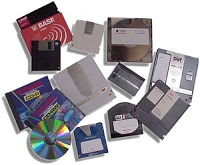
\includegraphics[width=180pt]{evidencia.jpg}
\end{figure}
\end{frame}

\subsection{�Confiar en lo electr�nico?}

\begin{frame}\frametitle{Confianza }


\begin{itemize}
\item Archivado - Guardado - Almacenamiento - Seguridad.\pause
\item Autenticidad - Fuerte y segura.\pause
\item Certificado Digital \pause
\item Claves privadas y Publicas \pause
\item Confianza Digital \pause
\end{itemize}
\end{frame}



\section{Confianza Digital}

\subsection{Confianza Digital}
\begin{frame}\frametitle{Confianza }
\begin{itemize}
\item �C�mo asegurar la identificaci�n de aquellos que est�n trabajando en un entorno digital o electr�nico?\pause
\item �C�mo asegurar la integridad de los datos y documentos enviados a trav�s de medios digitales?\pause
\item �C�mo conservar la confidencialidad de la informaci�n y los datos intercambiados o almacenados en un medio electr�nico?\pause
\item �C�mo crear un v�nculo claro entre un documento o una acci�n electr�nicos y la responsabilidad individual legal?
\end{itemize}
\end{frame}

\subsection{MD5}
\begin{frame}\frametitle{MD5}

\begin{figure}[h]

\includegraphics[width=100pt]{md5.jpg}
\end{figure}

\begin{itemize}
\item MD5 (abreviatura de Message-Digest Algorithm 5, Algoritmo de Resumen del Mensaje 5) es un algoritmo de reducci�n criptogr�fico de 128 bits.
\bigskip
\end{itemize}
\end{frame}

%SEGUNDO%

\subsection{Firmas Digitales}
\begin{frame}\frametitle{ Certificado Digital }


\begin{figure}[h]
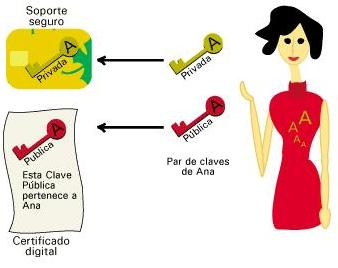
\includegraphics[width=200pt]{certificado.jpg}
\end{figure}

\end{frame}

\subsection{Estampa de Tiempo}
\begin{frame}\frametitle{Time Stamp}

\begin{itemize}
\item Marca de tiempo � Timestamping consiste en certificar mediante una secuencia de caracteres que un conjunto de datos ha existido y no ha sido modificado en un espacio de tiempo determinado. La secuencia de caracteres est� relacionada con la fecha y el momento en que ocurre dicho evento y espec�ficamente cuando fue creado en un sistema de c�mputo.\pause
\bigskip
\begin{figure}[h]

\includegraphics[width=120pt]{timestamp.jpg}
\end{figure}
\end{itemize}
\end{frame}

\begin{frame}\frametitle{Caracter�sticas }
\begin{itemize}
\item Certifica la hora y momento espec�fico en el que se lleva a cabo un suceso o se firma un archivo.\pause
\item Registra todo estampado de tiempo ocurrido, en una base de datos.\pause
\item Asegurar que no se altera el car�cter de confidencialidad del archivo\pause
\item Invalidar el sellado de tiempo si se altera el documento.
\end{itemize}
\end{frame}


\begin{frame}\frametitle{Beneficios }
\begin{itemize}
\item Minimiza el riesgo de modificaci�n de la informaci�n.\pause
\item Alteraci�n.\pause
\item Se eliminan factores de duda respecto del momento en que suceden acciones.
\end{itemize}
\end{frame}




\begin{frame}\frametitle{Y ahora todo eso de que me sirve?}
\begin{figure}[h]

\includegraphics[width=200pt]{info.jpg}
\end{figure}
\end{frame}

\section{Usando herramientas}
\subsection{Que hacemos ahora}

\begin{frame}\frametitle{A ponerlo en pr�ctica }
\begin{figure}[h]

\includegraphics[width=200pt]{garfield.jpg}
\end{figure}
\end{frame}

\subsection{Web Sellada}
\begin{frame}\frametitle{Web Sellada}
\begin{figure}[h]
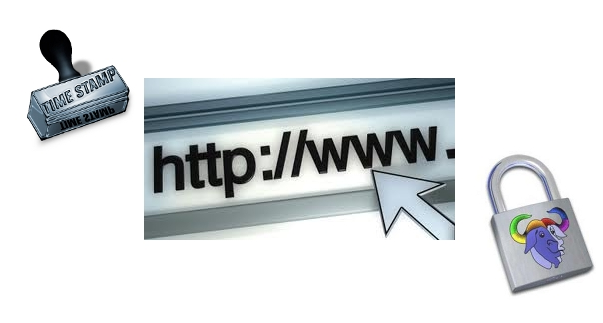
\includegraphics[width=280pt]{websellada.png}
\end{figure}
\end{frame}

\begin{figure}[h]
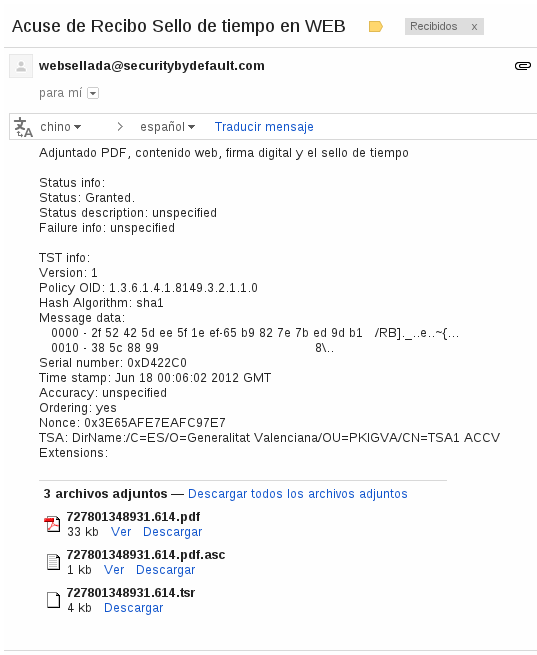
\includegraphics[width=180pt]{websellada2.png}
\end{figure}
\end{frame}

\begin{frame}\frametitle{Como se usa}
\begin{itemize}
\item Enviar un mail a websellada@securitybydefault.com \pause
\item url
\begin{figure}[h]
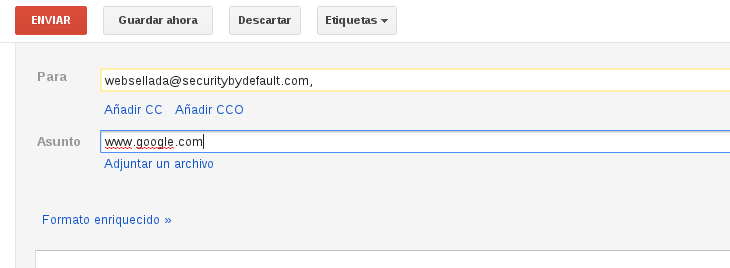
\includegraphics[width=120pt]{webselladamail.png}
\end{figure}
\end{itemize}
\end{frame}

\subsection{Mail Sellado}

\begin{frame}\frametitle{Mail Sellado}
\begin{figure}[h]
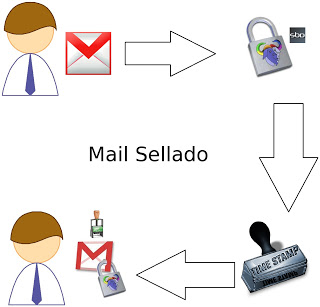
\includegraphics[width=100pt]{mailsellado2.jpg}
\end{figure}
\end{frame}

\begin{frame}\frametitle{Como se usa}
\begin{itemize}
\item Enviar un mail a websellada@securitybydefault.com \pause
\item url
\begin{figure}[h]
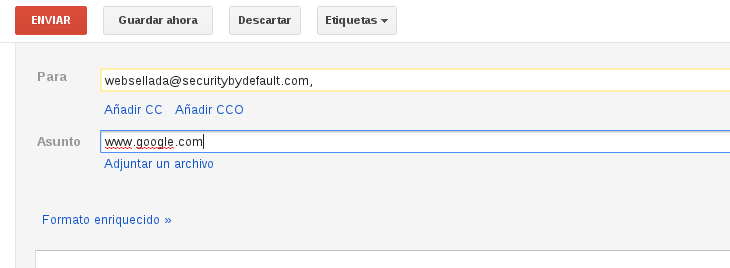
\includegraphics[width=120pt]{webselladamail.png}
\end{figure}
\end{itemize}
\end{frame}






\section{Preguntas} \label{Preguntas}



\begin{frame}\frametitle{Preguntas!}
\begin{figure}[h]

\includegraphics[width=160pt]{preguntas.jpg}
\end{figure}
\end{frame}



\end{document}

